\subsection{Background}
\subsubsection{Pearson Product-Moment correlation coefficient}

The Pearson product-moment correlation coefficient (or Pearson correlation coefficient, for short) is a measure of the strength of a linear association between two variables and is denoted by $r$.
Basically Pearson correlation coefficient, r, indicates how far away all these data points are to this line of best fit (how well the data points fit this new model/line of best fit).
Pearson correlation coefficient, r, represented with the following formula for populations:

$$ \rho_{X,Y} = \frac{cov(X,Y)}{\sigma_x \sigma_y}$$

Where $\sigma$ is a standard deviation of population and $cov$ is its covariance.
It can be also represented using the following formula for samples of size $n$:

$$r = \frac{\sum_{i=1}^{n} (X_i - \bar{X}) (Y_i - \bar{Y}) }
{ \sqrt{\sum_{i=1}^{n} (X_i - \bar{X})^2} \sqrt{\sum_{i=1}^{n} (X_i - \bar{X})^2} }$$

Pearson correlation coefficient can take a range of values from +1 (inclusive) to -1 (inclusive).
A value of 0 indicates that there is no association between the two variables.
A value greater than 0 indicates a positive association; meaning, as the value of one variable increases, so does the value of the other variable.
A value less than 0 indicates a negative association; meaning, as the value of one variable increases, the value of the other variable decreases.

Exemplar Pearson correlation coefficients with graphical visualization are shown in Figure~\ref{fig:pearson_graph}.

\begin{figure}[h]
  \centering
  \captionsetup{justification=centering}
    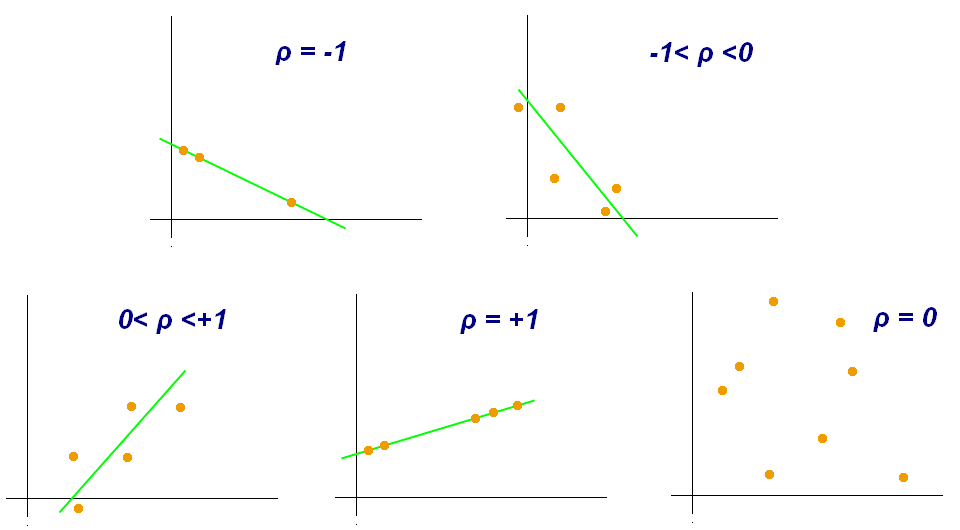
\includegraphics[width=0.8\textwidth]{images/pearson_graphs.png}
  \caption{Graphs showing dependence between graph points and line of best fit.\cite{wiki_pearson}}
  \label{fig:pearson_graph}
\end{figure}

\clearpage
One more thing to note regarding Pearson correlation coefficient is that it does not represent the slope of the line of best fit.
Therefore, if you get a Pearson correlation coefficient of +1 this does not mean that for every unit increase in one variable there is a unit increase in another.
It simply means that there is no variation between the data points and the line of best fit. This is illustrated below:

\begin{figure}[h]
  \centering
  \captionsetup{width=24pc, justification=centering}
    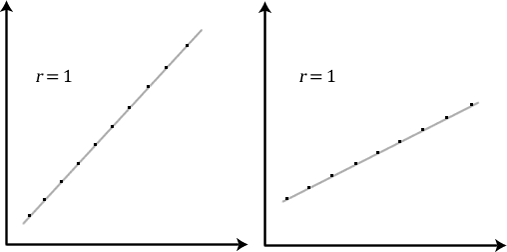
\includegraphics[width=0.55\textwidth]{images/pearson_graphs_slope.png}
  \caption{Graph showing independence of $r$ and slope of the line of best fit.}
  \label{fig:pearson_graph_slope}
\end{figure}